\lab{The Inverted Pendulum}{The Inverted Pendulum}
\label{lab:inverted_pendulum}
\labdependencies{IVPBVPIntro}

\objective{We will set up the LQR optimal control problem for the inverted pendulum and compute the solution numerically.
% We will add a stochastic component to the system.
}


Think back to your childhood days when, for entertainment purposes, you'd balance objects: a book on your head, a spoon on your nose, or even a broom on your hand.
 Learning how to walk was likely your initial introduction to the inverted pendulum problem.

A pendulum has two rest points: a stable rest point directly underneath the pivot point of the pendulum, and an unstable rest point directly above.
The generic pendulum problem is to simply describe the dynamics of the object on the pendulum (called the `bob').
The inverted pendulum problem seeks to guide the bob toward the unstable fixed point at the top of the pendulum.
Since the fixed point is unstable, the bob must be balanced relentlessly to keep it upright.

The inverted pendulum is an important classical problem in dynamics and control theory, and is often used to test different control strategies. One application of the inverted pendulum is the guidance of rockets and missiles. Aerodynamic instability occurs because the center of mass of the rocket is not the same as the center of drag. Small gusts of wind or variations in thrust require constant attention to the orientation of the rocket.


\section*{The Simple Pendulum}
We begin by studying the simple pendulum setting.
Suppose we have a pendulum consisting of a bob with mass $m$ rotating about a pivot point at the end of a (massless) rod of length $l$.
Let $\theta(t)$ represent the angular displacement of the bob from its stable equilibrium.
By Hamilton's Principle, the path $\theta$ that is taken by the bob minimizes the functional
\begin{align}
J[\theta] = \int_{t_0}^{t_1}	L,
\end{align}
where the Lagrangian $L = T - U$ is the difference between the kinetic and potential energies of the bob.

The kinetic energy of the bob is given by $mv^2/2$, where $v$ is the velocity of the bob.
In terms of $\theta$, the kinetic energy becomes
\begin{align}
	\begin{split}
	T &= \frac{m}{2}v^2  = \frac{m}{2}(\dot{x}^2 + \dot{y}^2),\\
	&= \frac{m}{2}((l\cos(\theta)\dot{\theta})^2 + (l\sin(\theta)\dot{\theta})^2),\\
	&= \frac{ml^2\dot{\theta}^2}{2}.
	\end{split}
\end{align}
The potential energy of the bob is $U = mg(l-l\cos \theta)$.
From these expressions we can form the Euler-Lagrange equation, which determines the path of the bob:
\begin{align}
	\begin{split}
	0 &= L_{\theta} - \frac{d}{dx}L_{\dot{\theta}},\\
	&= -mgl\sin \theta - m l^2 \ddot{\theta},\\
	&= \ddot{\theta} + \frac{g}{l}\sin \theta.
	\end{split}
\end{align}
Since in this setting the energy of the pendulum is conserved, the equilibrium position $\theta = 0$ is only Lyapunov stable. When forces such as friction and air drag are considered $\theta = 0$ becomes an asymptotically stable equilibrium.

%\begin{figure}
%\centering
%\includegraphics[width=8cm]{Simple_gravity_pendulum.png}
%\caption{The frame of reference for the simple pendulum problem.}
%\label{fig:inverted_pendulum:simple_gravity_pendulum}
%\end{figure}

\begin{figure}
\begin{center}
\begin{tikzpicture}

% Pole
\draw[ultra thick] (0,3.5) -- (1.2,1);
\filldraw[] (1.25,0.9) circle (0.25);

% Balancing line
\draw[very thin, dashed] (0,0.35) -- (0,3.5);

% Annotations
\draw[very thin] (0,2.8) arc (270:290:1);
\node[draw=none] at (0.2, 2.6){$\theta$};
\node[draw=none] at (0.9, 2.4){$l$};
\node[draw=none] at (1.35, 1.3){$m$};
\draw[<->, thin, >=stealth'] (-1.2,1.2) arc (252:288:3.5);

\end{tikzpicture}
\end{center}
\caption{The frame of reference for the simple pendulum problem.}
\label{fig:inverted_pendulum:simple_gravity_pendulum}
\end{figure}

\section*{The Inverted Pendulum}
\subsection*{The Control System}
We consider a gift suspended above a rickshaw by a (massless) rod of length $l$.
The rickshaw and its suspended gift will have masses $M$ and $m$ respectively, $M > m$.
Let $\theta $ represent the angle between the gift and its unstable equilibrium, with clockwise orientation.
Let $v_1$ and $v_2$ represent the velocities of the rickshaw and the gift, and $F$ the force exerted on the rickshaw.
The rickshaw will be restricted to traveling along a straight line (the $x$-axis).

By Hamilton's Principle, the path $(x,\theta)$ of the rickshaw and the present minimizes the functional
\begin{align}
J[x,\theta] = \int_{t_0}^{t_1}	L,
\end{align}
where the Lagrangian $L = T - U$ is the difference between the kinetic energy of the present on the pendulum, and its potential energy.

Since the position of the rickshaw and the present are $(x(t),0)$ and $(x-l\sin \theta, l\cos \theta)$ respectively, the total kinetic energy is
\begin{align}
	\begin{split}
	T &= \frac{1}{2}Mv_1^2 +  \frac{1}{2}mv_2^2\\
	&= \frac{1}{2}M\dot{x}^2 +  \frac{1}{2}m\left((\dot{x} - l\dot{\theta}\cos \theta)^2 + (- l\dot{\theta}\sin \theta)^2\right)\\
	&= \frac{1}{2}(M+m)\dot{x}^2 +\frac{1}{2}m l^2\dot{\theta}^2-ml\dot{x}\dot{\theta}\cos \theta.
	\end{split}
\end{align}

\noindent where $v_1$ is the norm of the velocity vector of the rickshaw and $v_2$ is that of the present.

% The potential energy $U$ is composed of two parts: the first is the gravitational potential energy of the bob/present on the pendulum, and is given by $(mg)(l\cos \theta)$.
% The second part is the potential energy in the system due to any force $F$ exerted on the rickshaw.
% Recalling that whenever a force field $\mathbf{F}$ has the form $\mathbf{F} = \nabla \phi(\mathbf{x})$, where $\phi(\mathbf{x})$ is a scalar field, the potential energy derived from that force is $ -\phi(\mathbf{x})$.
The total potential energy is
\begin{align*}
U &= mgl\cos \theta.
\end{align*}

\begin{figure}
\centering
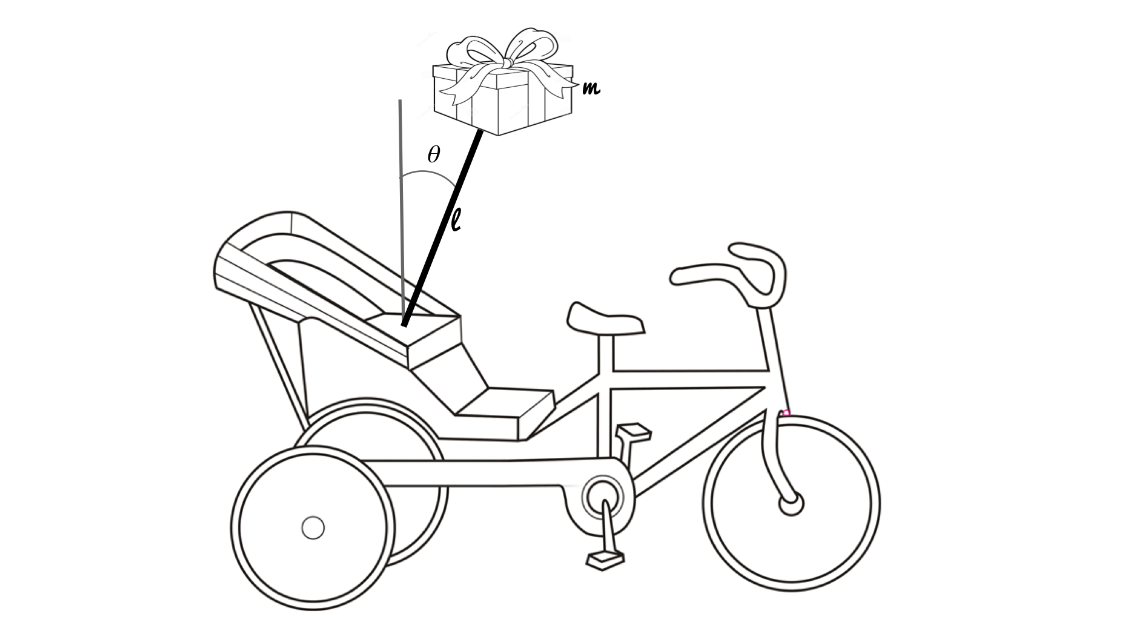
\includegraphics[width=\textwidth]{figures/rickshaw_img.png}
\caption{The inverted pendulum problem on a mobile rickshaw with a present suspended above.
}
\label{fig:inverted_pendulum:rickshaw_diagram}
\end{figure}

The path $(x,\theta)$ of the rickshaw and the present satisfy the Euler-Lagrange differential equations, but the problem involves a nonconservative force $F$ acting in the $x$ direction.
By way of D'Alambert's Principle, our normal Euler-Lagrange equations now include the nonconservative force $F$ on the right side of the equation:

\begin{align}
	\begin{split}
\frac{\partial L}{\partial x} - \frac{d}{dt} \frac{\partial L}{\partial \dot{x}} &= F,\\
\frac{\partial L}{\partial \theta} - \frac{d}{dt} \frac{\partial L}{\partial \dot{\theta}} &= 0.
	\end{split}\label{inverted_pendulum:langrange_eqns}
\end{align}
After expanding \eqref{inverted_pendulum:langrange_eqns} we see that $x(t)$ and $\theta(t)$ satisfy
\begin{align}
	\begin{split}
		F &= ml\ddot{\theta} \cos \theta - (M + m)\ddot{x} - ml \dot{\theta}^2 \sin \theta,\\
		l \ddot{\theta} &= g \sin \theta + \ddot{x} \cos \theta.
	\end{split}\label{inverted_pendulum:langrange_eqns_explicit}
\end{align}

At this point we make a further simplifying assumption.
If $\theta$ starts close to $0$, we may assume that the corresponding force $F$ will keep $\theta$ small.
In this case, we linearize\footnote{See Additional Material section for derivation.} \eqref{inverted_pendulum:langrange_eqns_explicit} about $(\theta, \dot{\theta}) = (0,0)$, obtaining the equations
\begin{align*}
	\begin{split}
		F &= ml\ddot{\theta} - (M + m)\ddot{x},\\
		l \ddot{\theta} &= g \theta + \ddot{x}.
	\end{split}%\label{inverted_pendulum:langrange_eqns_explicit2}
\end{align*}
These equations can be further manipulated
 % \eqref{inverted_pendulum:langrange_eqns_explicit2}
to obtain
\begin{align}
	\begin{split}
		\ddot{x} &=  - \frac{1}{M}F + \frac{m}{M}g\theta,\\
		\ddot{\theta} &= -\frac{1}{Ml}F + \frac{g}{Ml} (M+m) \theta.
	\end{split}\label{inverted_pendulum:langrange_eqns_explicit3}
\end{align}

We will now write \eqref{inverted_pendulum:langrange_eqns_explicit3} as a first order system.
Making the assignments $x_1 = x$, $x_2 = x_1'$, $\theta_1 = \theta$, $\theta_2 = \theta_1'$, letting $u = -F$ represent the control variable, we obtain
\begin{align*}
\begin{bmatrix}
x_1\\
x_2 \\
\theta_1 \\
\theta_2
\end{bmatrix}' &=
\begin{bmatrix}
0 & 1 & 0 & 0\\
0 & 0 & \frac{mg}{M} & 0 \\
0 & 0 & 0 & 1 \\
0 & 0 & \frac{g}{Ml}(M+m) & 0
\end{bmatrix}
\begin{bmatrix}
x_1\\
x_2 \\
\theta_1 \\
\theta_2
\end{bmatrix} + u
\begin{bmatrix}
0\\
\frac{1}{M} \\
0 \\
\frac{1}{Ml}
\end{bmatrix},
\end{align*}
which can be written more concisely as
\[z' = Az + Bu.\]

\subsection*{The Infinite Time Horizon LQR Problem}
We consider the cost function
\begin{align}
\begin{split}
J[z] &= \int_0^{\infty} (q_1x_1^2 + q_2x_2^2  + q_3\theta_1^2 + q_4\theta_2^2 + ru^2)\, dt\\
&= \int_0^{\infty} z\trp Qz + u\trp Ru \, dt
\end{split} \label{inverted_pendulum:LQR}
\end{align}
where $q_1, q_2, q_3, q_4$, and $r$ are nonnegative weights, and
\[
Q =
\begin{bmatrix}
q_1 & 0 & 0 & 0 \\
0 & q_2 & 0 & 0\\
0 & 0 & q_3 & 0 \\
0 & 0 & 0 & q_4
\end{bmatrix}, \quad R = \begin{bmatrix} r \end{bmatrix}.
\]

\begin{problem}
Write a function that returns the matrices $A, B, Q$, and $R$ given above. Let $g = 9.8\text{ m}/\text{s}^2$.

\begin{lstlisting}
def linearized_init(M, m, l, q1, q2, q3, q4, r):
	'''
	Parameters:
	----------
	M, m: floats
          masses of the rickshaw and the present
	l 	: float
          length of the rod
	q1, q2, q3, q4, r : floats
         relative weights of the position and velocity of the rickshaw, the
		 angular displacement theta and the change in theta, and the control

	Return
	-------
	A : ndarray of shape (4, 4)
	B : ndarray of shape (4, 1)
	Q : ndarray of shape (4, 4)
	R : ndarray of shape (1, 1)
	'''
	pass
\end{lstlisting}
\end{problem}

The optimal control problem \eqref{inverted_pendulum:LQR} is an example of a Linear Quadratic Regulator (LQR), and is known to have an optimal control $\tilde{u}$ described by a linear state feedback law:
\begin{align*}
\tilde{u} &= -R^{-1}B\trp P\tilde{z}.
\end{align*}
Here $P$ is a matrix function that satisfies the Riccati differential equation (RDE)
\[
\dot{P}(t) = PA + A\trp P + Q - PBR^{-1}B\trp  P.
\]
Since this problem has an infinite time horizon, we have $\dot{P} = 0$. Thus $P$ is a constant matrix, and can be found by solving the algebraic Riccati equation (ARE)
\begin{align}
 PA + A\trp P + Q - PBR^{-1}B\trp  P = 0.  \label{inverted_pendulum:ARE}
\end{align}
The evolution of the optimal state vector $\tilde{z}$ can then be described by \footnote{See Calculus of Variations and Optimal Control Theory, Daniel Liberzon, Ch.6}
\begin{align}
\dot{\tilde{z}} = (A - BR^{-1}B\trp P)\tilde{z}. \label{inverted_pendulum:optimal_state}
\end{align}

\begin{problem}
Write the following function to find the matrix $P$.
Use \li{scipy.optimize.root}.
Since \li{root} takes in a vector and not a matrix, you will have to reshape the matrix $P$ before passing it in and after getting your result, using \li{P.reshape(16)} and \li{P.reshape((4,4))}.
\begin{lstlisting}
def find_P(A, B, Q, R):
	'''
	Parameters:
	----------
	A, Q 	: ndarrays of shape (4, 4)
	B		: ndarray of shape (4, 1)
	R		: ndarray of shape (1, 1)

	Returns
	-------
	P		: the matrix solution of the Riccati equation
	'''
	pass

\end{lstlisting}
Using the values
\begin{lstlisting}
M, m = 23., 5.
l = 4.
q1, q2, q3, q4 = 1., 1., 1., 1.
r = 10.
\end{lstlisting}
compute the eigenvalues of $A - BR^{-1}B\trp P$.
Are any of the eigenvalues positive?
Consider differential equation \eqref{inverted_pendulum:optimal_state} governing the optimal state $\tilde{z}$.
Using this value of $P$, will we necessarily have $\tilde{z} \to 0$?
\end{problem}

\begin{problem}
	Write the following function that implements the LQR solution described earlier.
	Use \li{scipy.integrate.solve_ivp} to solve the IVP.
\begin{lstlisting}
def rickshaw(tv, X0, A, B, Q, R, P):
	'''
	Parameters:
	----------
	tv 	: tuple containing the start and end times (t0, tf) that can be passed into solve_ivp
	X0 	: Initial conditions on state variables
	A, Q: ndarrays of shape (4, 4)
	B	: ndarray of shape (4, 1)
	R	: ndarray of shape (1, 1)
	P	: ndarray of shape (4, 4)

	Returns
	-------
	Z : ndarray of shape (n+1, 4), the state vector at each time
	U : ndarray of shape (n+1,), the control values
	'''
	pass
\end{lstlisting}
\label{prob:inverted_pendulum3}
\end{problem}


Notice that we have no information on how many solutions \eqref{inverted_pendulum:ARE} possesses.
In general there may be many solutions.
We hope to find a unique solution $P$ that is \textit{stabilizing}: the eigenvalues of $A - BR^{-1}B\trp P$ have negative real part.
To find this $P$, use the function \li{solve_continuous_are} from \li{scipy.linalg}.
This function is designed to solve the continuous algebraic Riccati equation.


\begin{problem}
Test the function made in Problem \eqref{prob:inverted_pendulum3} with the following inputs:
\begin{lstlisting}
M, m = 23., 5.
l = 4.
q1, q2, q3, q4 = 1., 1., 1., 1.
r = 10.
tf = None
X0 = np.array([-1, -1, .1, -.2])
\end{lstlisting}
Find the matrix P using the \li{scipy.optimize.root} method with \li{tf=6} as well as the

\noindent \li{solve_continuous_are} method with \li{tf=60}.
Plot the solutions $\tilde{z}$ and $\tilde{u}$.
Your results should show behavior similar to that in Figure \ref{fig:inverted_pendulum:4}.
Be sure to include a legend.
% and \ref{fig:inverted_pendulum:prob4_stable} respectively.
\label{prob:inverted_pendulum:4}
\end{problem}

\begin{figure}
\begin{minipage}[b]{.47\linewidth}
\centering
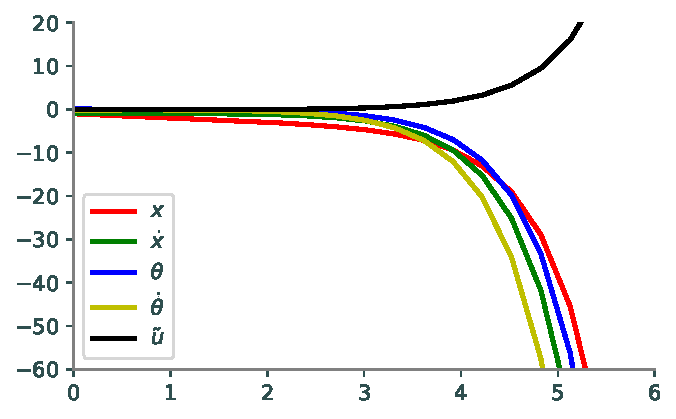
\includegraphics[width=\textwidth]{figures/prob4_unstable.pdf}
\caption*{$P$ is found using \li{scipy.optimize.root}.}
\end{minipage}
\hspace{0.5cm}
\begin{minipage}[b]{0.47\linewidth}
\centering
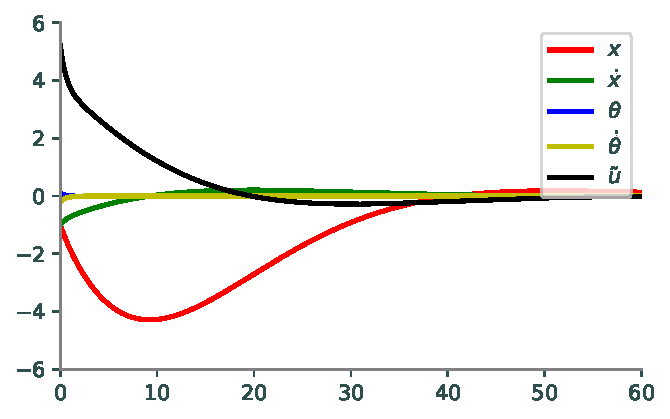
\includegraphics[width=\textwidth]{figures/prob4_stable.pdf}
\caption*{$P$ is found using \li{solve_continuous_are}.}
\end{minipage}
\caption{The solutions of Problem \ref{prob:inverted_pendulum:4}.}
\label{fig:inverted_pendulum:4}
\end{figure}

\begin{comment}
\begin{problem}
Consider the following inputs:
\begin{lstlisting}
M, m = 23., 5.
l = 4.
q1, q2, q3, q4 = 1., 1., 1., 1.
r = 10.
tf = 60
X0 = np.array([-1, -1, .1, -.2])
\end{lstlisting}
Vary the entries of \li{X0} responsible for $\theta(0)$ and $\dot{\theta}(0)$ to determine the sensitivity of the control $u$ to the initial conditions.  What initial conditions lead to a reasonable, physical control $u$? (Plot several solutions with various values of $\theta(0)$ and $\dot{\theta}(0)$.)
\end{problem}
\end{comment}

The LQR solution we have found only works for the linearized version of the ODE system that we found. What if we were to apply the control found in the LQR formulation to the original, nonlinear ODE found in \eqref{inverted_pendulum:langrange_eqns_explicit}?
To do this, we need to first be able to interpolate the control variable $u$ found in Problem \ref{prob:inverted_pendulum:4} using SciPy's \li{CubicSpline} function (see the \href{https://docs.scipy.org/doc/scipy/reference/generated/scipy.interpolate.CubicSpline.html}{documentation} for more details).
We also need to solve \eqref{inverted_pendulum:langrange_eqns_explicit} for $\ddot x$ and $\ddot \theta$. Note that $-F$ in \eqref{inverted_pendulum:langrange_eqns_explicit} is the control variable $u$ in \eqref{inverted_pendulum:langrange_eqns_solved}.


\begin{align}
	\begin{split}
		\ddot x &= \frac{u+m\sin\theta(-l\dot \theta^2+g\cos\theta)}{M+m(1-\cos^2\theta)},\\
		\ddot{\theta} &= \frac{g(m+M)\sin\theta+\cos\theta(u-lm\dot\theta^2\sin\theta)}{l(M+m(1-\cos^2\theta))}.
	\end{split}\label{inverted_pendulum:langrange_eqns_solved}
\end{align}

\begin{problem}
Using the same variables and initial conditions as in Problem \ref{prob:inverted_pendulum:4}, and the cubic spline interpolation of the control found in Problem \ref{prob:inverted_pendulum:4}, solve for the state variables $\tilde{z}$. Plot $\tilde{z}$, as well as the solution $\tilde{u}$ found in Problem \ref{prob:inverted_pendulum:4} with \li{tf=15}. Compare your results with the first image in Figure \ref{fig:nonlinear_inverted_pendulum:5}.
Notice that the initial $\theta$ is large enough that the inverted pendulum is not balanced. Instead, it falls over at about 5 seconds.


The problem is that the the linearized system is only a valid approximation of the true nonlinear system on small time intervals.
So let's solve for the optimal control of the linearized system one small interval at a time.

Starting with the initial condition given in Problem \ref{prob:inverted_pendulum:4}, use your \li{rickshaw} solver (from Problem \ref{prob:inverted_pendulum3}) to solve the linearized system over a small interval $t\in[t_0,t_1]$ and obtain the control $\tilde u$.
Interpolate this $\tilde u$ (again using \li{CubicSpline}), then use this interpolation to evolve the true nonlinear system on the same interval.
Now we repeat the process by taking the final state $\tilde z$ on this interval as our new initial condition for the next interval $t \in [t_1, t_2]$.
Plugging this initial condition into \li{rickshaw}, we obtain a control which we then interpolate and use to evolve the nonlinear system.
Continue this until you have solved over the entire time interval $t\in[0,60]$.

Plot the pieced-together $\tilde{z}$ and $\tilde{u}$.
Be sure to include a legend.
Compare your results with the second image in Figure \ref{fig:nonlinear_inverted_pendulum:5}.

Hint: use \li{np.geomspace(1,61,120)-1} to get a list of $\{t_0, t_1, ... t_f\}$ that will work well. Solving the equation more often at the beginning will keep the control variable approximately continuous. You only need to solve for the control $\tilde u$ at 3 points in each interval $[t_i, t_{i+1}]$ for the method to work well.
Also, use \li{solve_continuous_are} rather than \li{scipy.optimize.root} when solving the linearized system.

\label{prob:inverted_pendulum:5}
\end{problem}

\begin{figure}[H]
\begin{minipage}[b]{.47\linewidth}
\centering
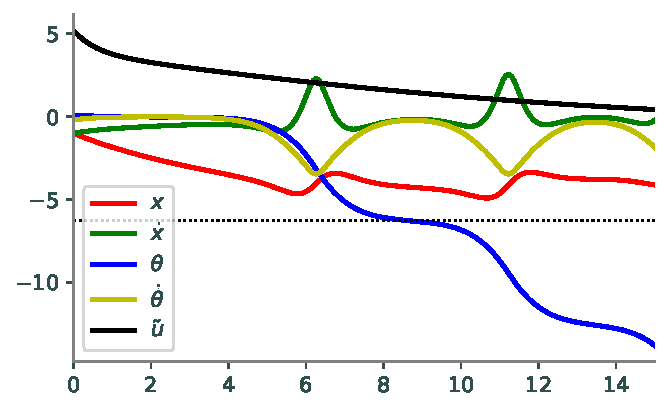
\includegraphics[width=\textwidth]{figures/nonlinear_attempt1.pdf}
\caption*{Resulting state equations if the linearized equation is only solved once before the $\theta$ is sufficiently small. Note that the pendulum falls and starts spinning at around 5 seconds. The pendulum makes a full revolution at about 9 seconds ($2\pi$ rotations is marked by the dotted line).}
\end{minipage}
\hspace{0.5cm}
\begin{minipage}[b]{0.47\linewidth}
\centering
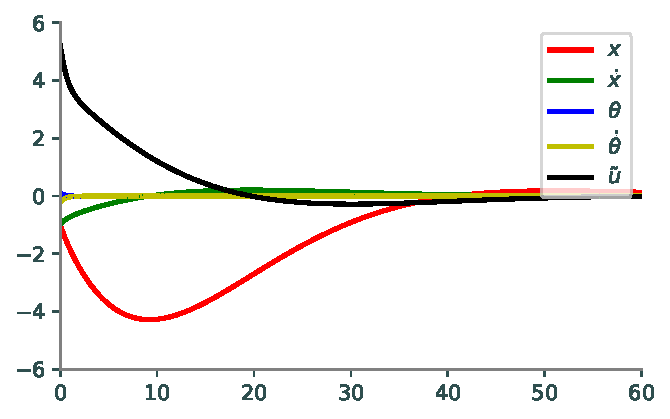
\includegraphics[width=\textwidth]{figures/nonlinear_attempt2.pdf}
\caption*{The resulting state equations if the linearized equation is solved again every two seonds. Note that when $\theta$ is larger in the first 2 seconds, the control is not sufficiently large. This is issue is resolved by solving the equation again at 2 seconds. Compare this solution to the second image in Figure \ref{fig:inverted_pendulum:4}}
\end{minipage}
\caption{The solutions of Problem \ref{prob:inverted_pendulum:5}.}
\label{fig:nonlinear_inverted_pendulum:5}
\end{figure}


\newpage

\section*{Additional Material} % ==============================================

\subsection*{Linearization} % -----------------------------------------------

Recall that a first-order Taylor approximation of a function $\f(\x)$, centered at $\x_0$, is

\begin{equation*}
\f(\x) \approx \f(\x_0) + D\f(\x_0) (\x - \x_0).
\end{equation*}

\noindent We linearize the right-hand sides of equations \eqref{inverted_pendulum:langrange_eqns_explicit} around $(\theta, \dot \theta) = (0, 0)$ as follows:

\begin{align*}
H_1(\theta, \dot \theta) &\coloneq ml\ddot{\theta} \cos \theta - (M + m)\ddot{x} - ml \dot{\theta}^2 \sin \theta\\
&\approx H_1(0, 0) + DH_1(0, 0)
    \begin{bmatrix}
        \theta - 0\\
        \dot \theta - 0
    \end{bmatrix}\\
&= m l \ddot \theta - (M + m) \ddot x\\
& \quad + \left[- m l \ddot \theta \sin \theta - m l \dot \theta^2 \cos \theta,
- 2 m l \dot \theta \sin \theta \right]
\bigg|_{(\theta, \dot \theta) = (0, 0)}
    \begin{bmatrix}
        \theta\\
        \dot \theta
    \end{bmatrix}\\
&= m l \ddot \theta - (M + m) \ddot x + \left[0, 0 \right]
    \begin{bmatrix}
        \theta\\
        \dot \theta
    \end{bmatrix}\\
&= m l \ddot \theta - (M + m) \ddot x.
\end{align*}

\noindent Similarly,

\begin{align*}
H_2(\theta, \dot \theta) &\coloneq g \sin \theta + \ddot x \cos \theta\\
&\approx H_2(0, 0) + DH_2(0, 0)
    \begin{bmatrix}
        \theta\\
        \dot \theta
    \end{bmatrix}\\
&= \ddot x + \left[g \cos \theta - \ddot x \sin \theta, \; 0\right]
\bigg|_{(\theta, \dot \theta) = (0, 0)}
    \begin{bmatrix}
        \theta\\
        \dot \theta
    \end{bmatrix}\\
&= \ddot x + \left[g, 0\right]
    \begin{bmatrix}
        \theta\\
        \dot \theta
    \end{bmatrix}\\
&= \ddot x + g \theta.
\end{align*}
